\documentclass[a4paper,12pt]{article}

\usepackage{préambule}
\usepackage{clipboard}

\begin{document}

\begin{center}
	\begin{Large}
		Grille exercice 4 \vspace{1em}
	\end{Large}

	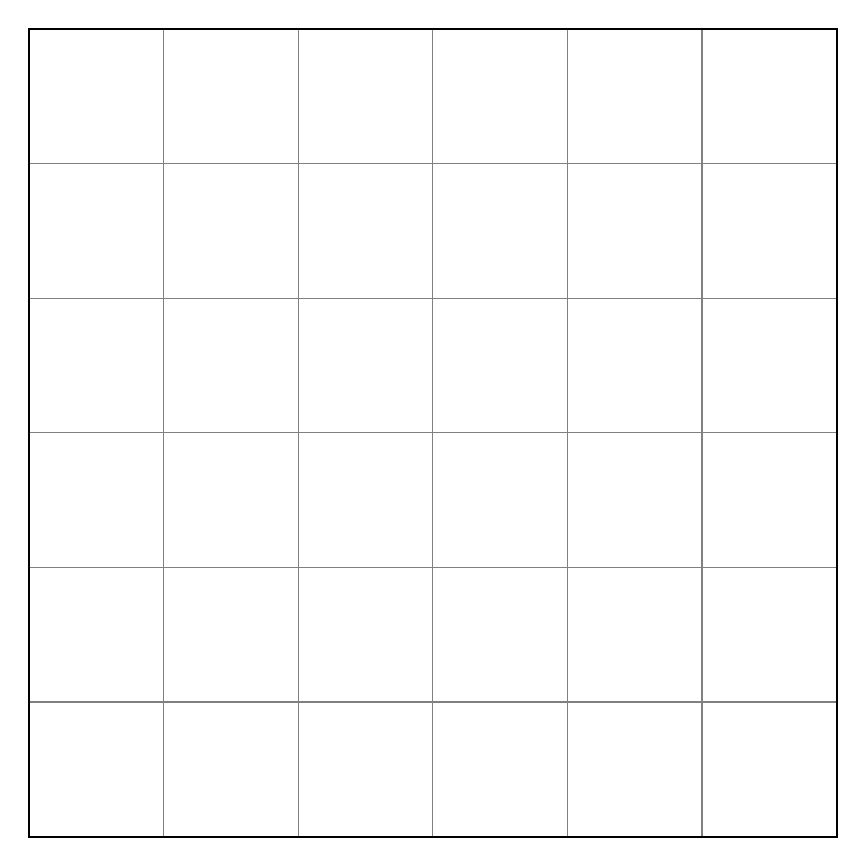
\begin{tikzpicture}[scale=1.71]
		\draw[step=1.0,gray,thin] (0,0) grid (6,6);
		\draw[black,thick] (0,0) rectangle (6,6);
	\end{tikzpicture}

	\vspace{3em}
	\hrule
	\vspace{3em}

	\begin{Large}
		Grille exercice 4 \vspace{1em}
	\end{Large}

	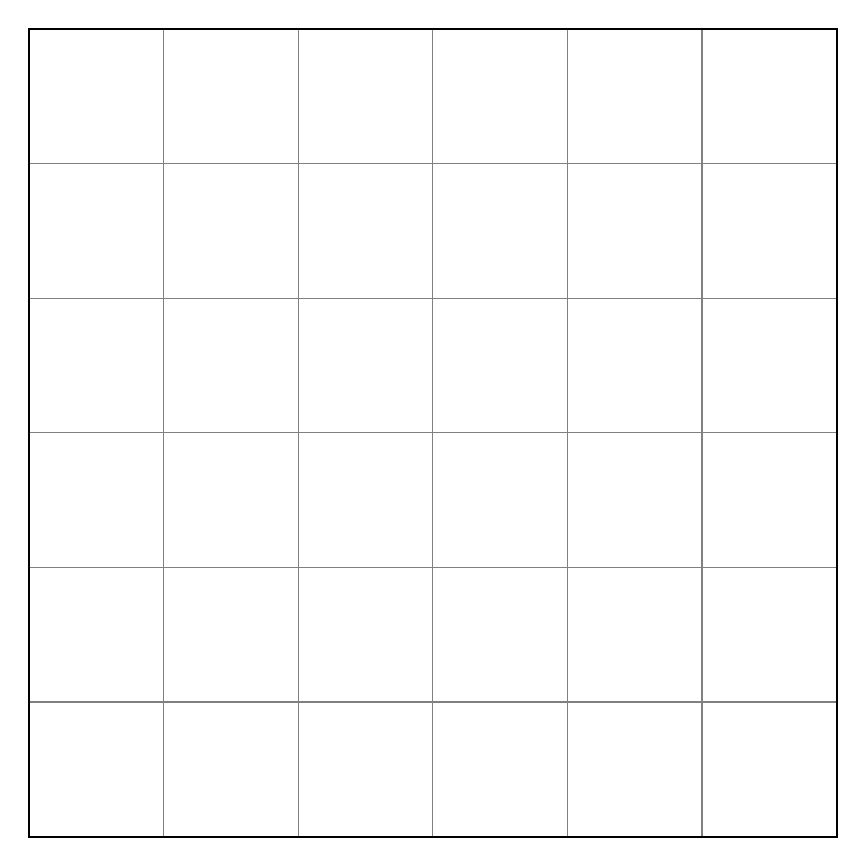
\begin{tikzpicture}[scale=1.71]
		\draw[step=1.0,gray,thin] (0,0) grid (6,6);
		\draw[black,thick] (0,0) rectangle (6,6);
	\end{tikzpicture}
\end{center}

\end{document}